\documentclass[12pt, a4paper, twoside, openright]{book}

\usepackage[french]{babel}
\usepackage[T1]{fontenc}
\usepackage[utf8]{inputenc}
\usepackage{lmodern}
\usepackage{graphicx}
\usepackage{hyperref}
\usepackage{listings}
\usepackage{graphicx}
\usepackage{microtype}
\usepackage{glossaries}
\makeglossaries %à la suite de la déclaration de package
\newacronym{sgbd}{Système de gestion de base de données}{Logiciel permettant...}



%define
\newcommand{\exemple}[1]{\newline\newline

\centering\parbox{5cm}{\textcolor{red}{#1}}

}
%end define

\title{Interfaces homme-machine pour gestion de bases de données.}
\author{ALCANTUD Gaël \\ BULATOVIC Alexandre \\ MAURY Adrian \\ UGOLINI Romain \\ \\tuteur : PALLEJA Xavier}
\date{20/02/2017}

\begin{document}
\frontmatter
\maketitle

\thispagestyle{empty}
\chapter*{Résumé}
\textbf{IDB} est un logiciel gratuit permettant d'utiliser un SGBD* au moyen d'une interface graphique. Son interface est intuitive et permet à un utilisateur, même non informaticien, de manipuler très facilement des tables et les données qu'elles contiennent, mais aussi d'effectuer des requêtes simples (en allant jusqu'aux jointures) sans se soucier du langage SQL*.
\\
Le logiciel est entièrement codé en langage Java (nécessite au minimum JRE* 1.7) et se base sur la bibliothèque JDBC* pour réaliser la communication avec la base de données. Il est entièrement compatible avec les système de gestion de base de données Oracle Database et MySQL.
\bigbreak
Mots clés : base de données, JAVA, JDBC, SQL, interface graphique, Oracle, MySQL, QBE

\bigbreak
\rule{\linewidth}{0.4pt}
\bigbreak

\textbf{IDB} is a free software intended to handle the administration of a database management system with the use of a GUI*. Its use is intuitive and allow non-IT people to manage tables and their data, but also to perform simple queries (even join clause) without having to know SQL*.
\\
This software is written in Java language (requires JRE* 1.7+) and uses the JDBC* tool from Java language to achieve communication with the database management system. It's fully compatible with Oracle Database and MySQL.
\bigbreak
Keywords : database, JAVA, JDBC, SQL, graphical user interface, Oracle, MySQL, QBE


\thispagestyle{empty}
\chapter*{Remerciements}



Premièrement nous tenons à remercier notre tuteur de projet, \textbf{M. Xavier PALLEJA}, pour avoir encadré ce projet et nous avoir guidé dans la réalisation de l'application à l'aide d'un cycle de développement itératif.

Nous apprécions grandement sa forte implication dans le projet et nous tenons à lui en faire part.

\bigbreak

Nous remercions également les différentes personnes travaillant à l'IUT nous ayant permis d'avancer le projet en mettant à disposition des salles informatiques, notamment les techniciens réseau.

\bigbreak
Enfin, nous remercions \textbf{M. Francis GARCIA} pour son rôle de chef de département informatique et d'avoir fait en sorte que tout se passe au mieux.

De même nous remercions notre professeur de communication \textbf{M. Alain RAIBAUT} pour ses cours qui nous ont été utile à la rédaction de ce rapport ainsi que les précieux conseils donnés sur la façon de gérer une présentation orale.


\tableofcontents
\listoffigures
\printglossaries

\mainmatter
\chapter*{Introduction}
Les \glspl{bdd} sont des outils permettant de stocker et retrouver des \glspl{data}, c'est à dire des valeurs brutes. 
Ces outils se trouvent au coeur des \glspl{si}, et sont indispensables aux entreprises.

En informatique, les bases de données sont numérisées, définies et manipulées grâce à des logiciels nommés \glspl{sgbd}.

Il existe différents types de bases de données, mais le marché reste dominé par les \glspl{bddr}\footnote{\label{part_de_marché_relationnel}
Classement des \glspl{sgbd} les plus populaires : \url{http://db-engines.com/en/ranking}}. Ces dernières sont gérées par des SGBD relationnels (dit SGBDR) 
dont les plus connus sont Oracle, MySQL et PostgreSQL.

Ces logiciels permettent de définir et de manipuler des bases de données par le biais du \gls{sql}, 
langage déclaratif et normé qui reste le premier et le plus exhaustif des moyens de gérer une base de données relationnelle .

Mais le SQL est un langage informatique, ce qui constitue un frein pour les utilisateurs : s'ils ne connaissent pas
le langage, ils ne peuvent pas utiliser de base de données.

Certaines applications, comme \textit{Access}, \textit{LOBase} ou encore \textit{phpMyAdmin} proposent une alternative au SQL grâce à des 
\glspl{ihm}: il est possible de définir les données ou de les manipuler par des clics de boutons, des glisser-déplacer, des cases à cocher ou encore de la saisie
de texte non codé. 

En suivant cette optique, le but de ce projet tuteuré est de réaliser une application permettant d'utiliser certaines fonctionnalités 
des bases de données \underline{sans} 
avoir recours au SQL, et ce sur n'importe quel SGBDR. Pour cela, elle propose une série d'IHM qui en reprennent certaines fonctionnalités,
à savoir le \gls{ldd} et le \gls{lmd}.

Les utilisateurs finaux de l'application sont les élèves de première année du DUT Informatique, pour
les aider à découvrir les bases de données.

Ce document présente les différentes phases de création de cette application : l'analyse, la conception, le développement et les tests.
Un manuel d'utilisation est disponible dans les dernières pages.

Afin de mieux situer l'application, la figure \ref{sans_idb_schema} montre l'utilisation classique d'un SGBD et 
la figure \ref{avec_idb_schema} l'utilisation de l'application développée.

\begin{figure}[!h]
  \centering
  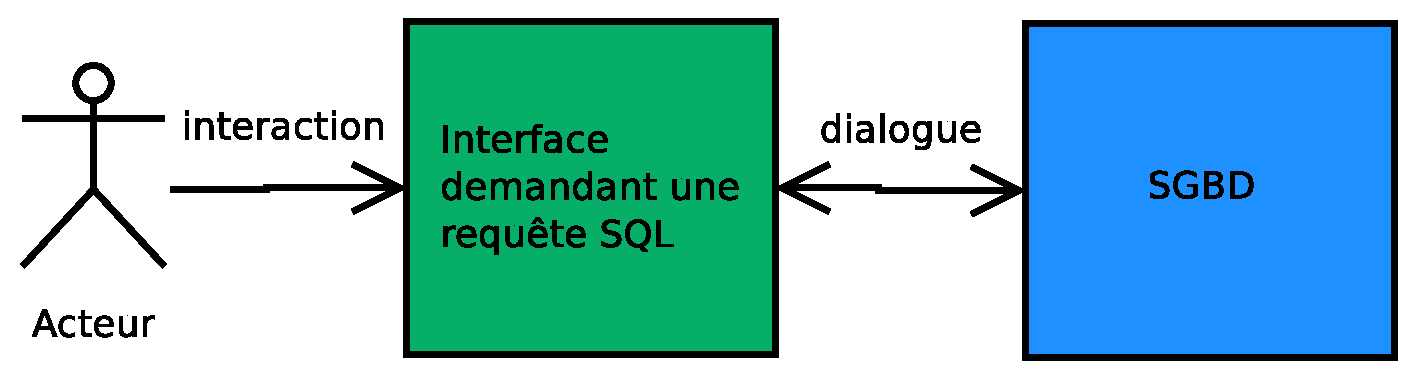
\includegraphics[width=14cm]{images/sans_idb.eps}
  \caption{Utilisation classique d'un SGBD.}
  \label{sans_idb_schema}
\end{figure}

\begin{figure}[!h]
  \centering
  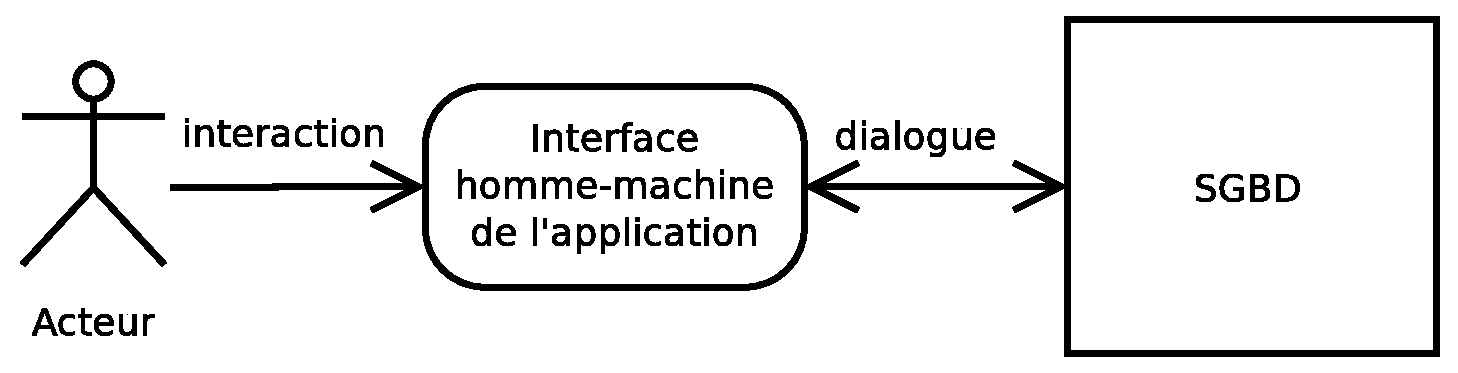
\includegraphics[width=14cm]{images/avec_idb.eps}
  \caption{Utilisation d'un SGBD avec l'application du projet.}
  \label{avec_idb_schema}
\end{figure}
%TODO : donner un nom à l'application


\backmatter

\end{document}
